\documentclass[crop,tikz,border=1px]{standalone}

\usetikzlibrary{arrows,positioning,scopes,automata,calc}

\begin{document}
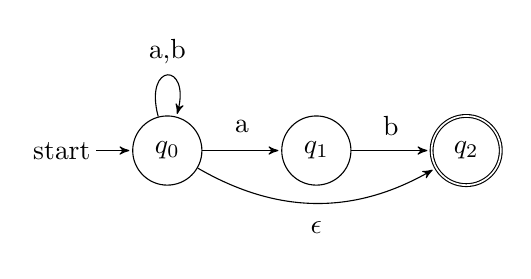
\begin{tikzpicture}[->,>=stealth',shorten >=1pt,auto,
  inner sep=2pt,minimum size=.6cm,
  mystate/.style={state,text centered}]

  \node[initial,mystate] (q0) {\(q_0\)};
  \node[mystate] (q1) [right=of q0] {\(q_1\)};
  \node[accepting,mystate] (q2) [right=of q1] {\(q_2\)};

  \path (q0) edge [loop above] node [above] {a,b} (q0)
        (q0) edge node [above] {a} (q1)
        (q1) edge node [above] {b} (q2)
        (q0) edge [bend right] node [below] {\(\epsilon\)} (q2);

\end{tikzpicture}
\end{document}
